
%(BEGIN_QUESTION)
% Copyright 2014, Tony R. Kuphaldt, released under the Creative Commons Attribution License (v 1.0)
% This means you may do almost anything with this work of mine, so long as you give me proper credit

Beregn kildestrømmen og laststrømmen i denne transformatorkretsen:

$$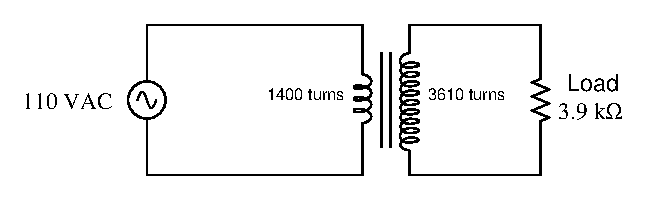
\includegraphics[width=15.5cm]{i01255x01.eps}$$

$I_{kilde}$ = \hskip 80pt $I_{last}$ =

\vskip 10pt

\underbar{file i01255}
%(END_QUESTION)





%(BEGIN_ANSWER)

$I_{kilde}$ = 187.5 mA \hskip 80pt $I_{last}$ = 72.73 mA

%(END_ANSWER)





%(BEGIN_NOTES)

De fleste transformatorproblemer er ikke noe mer enn forholdsregning, men noen studenter synes forhold er vanskelige å håndtere. Spørsmål som dette er flotte for å få studenter til å komme opp til tavlen foran i klasserommet og demonstrere hvordan de kom frem til resultatene.

%INDEX% Electronics review: transformer ratios

%(END_NOTES)
